\chapter{Hardware}
\section{Sensors}
\subsection{Lidar}

\subsection{Radar}
\subsubsection{Mount}
\subsection{IMU}
\section{Husky A200}
\subsection{Kinematics}
\section{Computers}


\chapter{Theory}
\section{Tools}
This section will explain the tools used in this project, like ROS, ubuntu, the lidar radars husky....
\section{ROS system}
The work done in this project is a continuation and expansion of previous work \ref{Appdix:MAS513}. This previous work consisted of, among other things, configuring a Unmanned Ground Vehicle (UGV) along with sensors, in ROS2. There was therefore a desire to continue the work in this project in ROS2. The issue was that the pre-made package for the radar-modules was made for ROS1. The migration methods described on the official ROS2 documentation where attempted (described in \cite{ROSMigrationGuide}). Attempts where also made on using Amazon's tools for migrating ROS1 to ROS2 (described in \cite{ROSMigrationGuide}). Attempts on migrating the radar-package to ROS2 was ultimately abandoned. The perception system was implemented i ROS1, then the ROS1 bridge was utilised for communicating with the rest of the system which runs on ROS2.

\subsection{ROS1 system}
The ROS1 system is responsible for reading in data from a 3D-Lidar \ref and two radar-modules \ref, combining data and sending it on a format can be used for navigation purposes. The navigation system used in this project, and in \ref{Appdix:MAS513}, relays on the Laserscan message sent on the "/scan"-topic. The ROS1 system must provide the ROS2 system with the proper messages on the "/scan"-topic. Figure \ref{fig:rqt:ros1_noBridge} displays a rqt node-graph of the ROS1 system. The system is divided in to four main parts, which will be explained in the following parts.

Figure \ref{fig:simpleRos1Rqt} simplified presentation of the visualisation system running on ROS1. The nodes are represented by the red ovals, the green rectangles depicts the topics and the blue rectangles are used for groups, or common name spaces. All of the nodes, topics and "groups" that exists in a group share a common name space, like "$/namespace"$. For example, all the entities in the "$/radar0$" group begin their name with "$/radar0$". This naming convention serves two purposes, it allows , in a way, all the sensors to publish to the same topic name. For example, all of the sensors publishes to the "$/PointCloud$" topic, but no issues with similar names arises because they all use different naming prefixes. The second purpose is to allow the system to be viewed in a intuitive and structured way in the rqt node-graph.  

\begin{figure}[H]
\centering
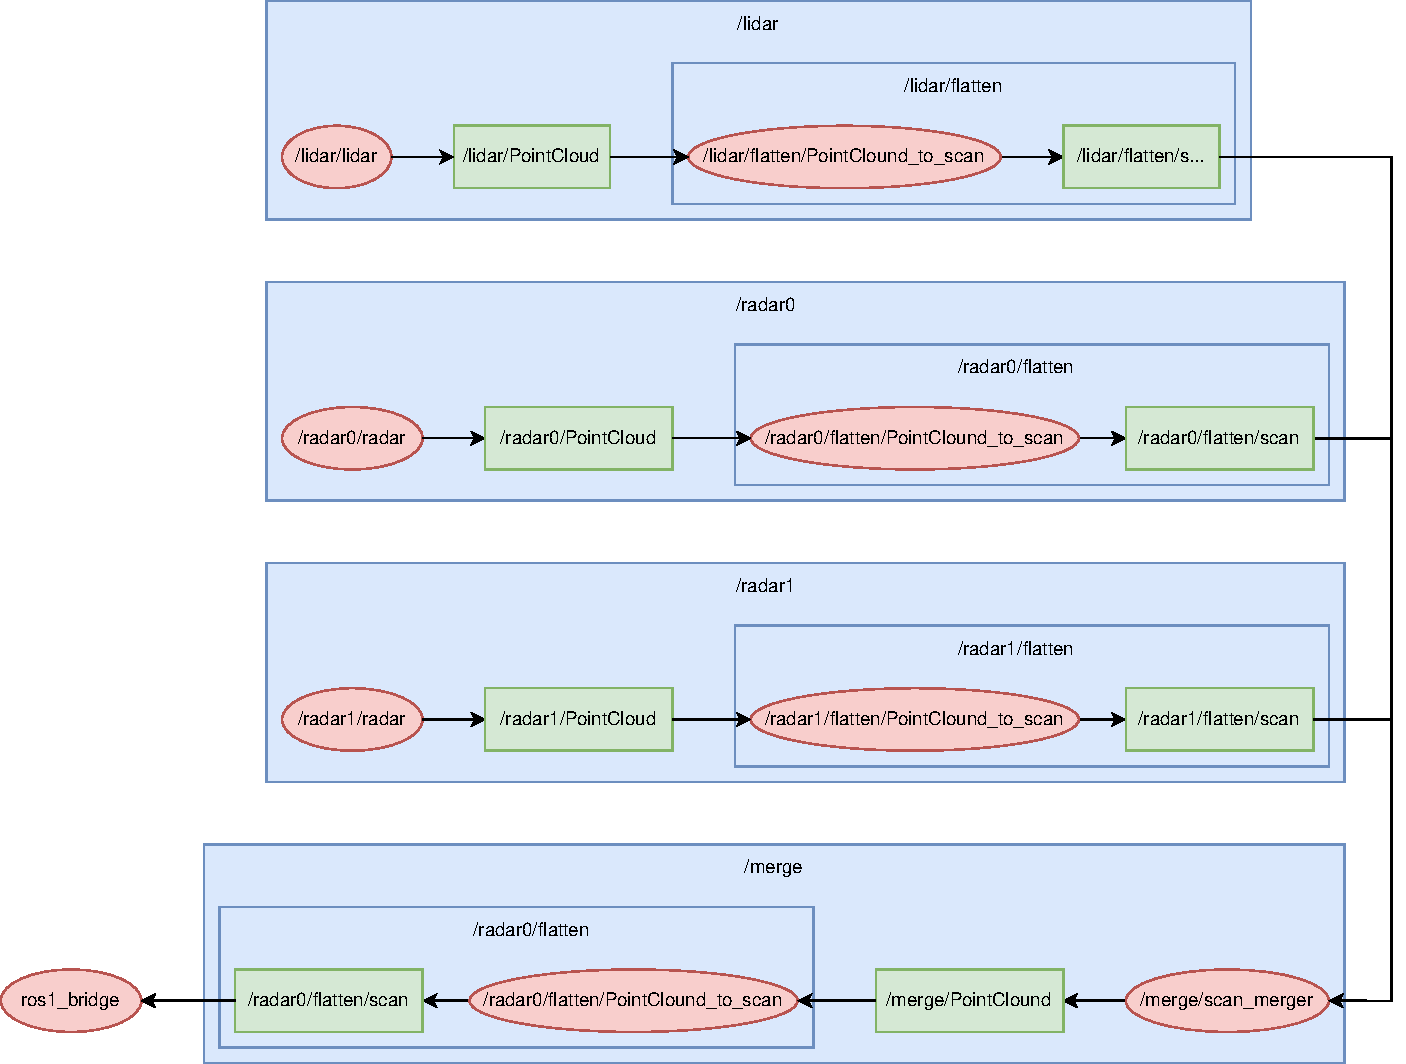
\includegraphics[scale=0.65]{Figures/draw.io/sipleRqtRos1.drawio.pdf}
  \caption{Simplifyed node-graph of ROS1 system}
  \label{fig:simpleRos1Rqt}
\end{figure}
%\subsection{Launch files}

The system is brought up with the help of launch files. One launch file (two in practice) is used to launch the entire ROS1 system, except the ROS1 bridge. The master launch file(s) are responsible for calling upon other "sublaunch" files. The sublaunch file system allows similar functionality to be re-used, similarly to how functions might be used in c or Python. All of the groups depicted in figure \ref{fig:simpleRos1Rqt} has a sublaunch file associated with it. 

The sublaunch files takes in arguments, which can be passed over to the elements being launched. The arguments can be passed to the sublaunch file when it is called, but there are default settings that are applied for the arguments not specified when the launch file is ran. The arguments are passed down either to the nodes or the launch files that are called upon. Some of the arguments are used so that one launch file can called by different launch files without them interfering with each other, by for example changing the prefix on nodes and topics, like mentioned above. The following sections will go over the different sublaunch files used by the main launch file(s)

\subsubsection{\textit{flatten.launch}}\label{subsubsec:flatten.launch}
"\textit{flatten.launch}" is used to launch the \textit{pointcloud\_to\_laserscan\_node} 
node of the \textit{pointcloud\_to\_laserscan} package. The \textit{pointcloud\_to\_laserscan\_node} node is used to convert a 3D point cloud to a 2D laser scan \cite{pcl_ros}. The conversion will include objects within a given height range set by two arguments, "\textit{min\_height}" and "\textit{max\_height}". The \textit{pointcloud\_to\_laserscan\_node} node subscribes to the \textit{cloud\_in} topic, and expect a message on the \textit{sensor\_msgs/PointCloud2} message format \cite{pcl_ros}. \textit{remap} is used to make the node more generic by allowing the subscribed topic to be set by an argument. The node publishes on the \textit{scan} topic with the \textit{sensor\_msgs/LaserScan} message format. The node is launched within a group with a name space (NS) which adds a NS prefix to the name of the launched node and the published topic.

\subsubsection{\textit{lidar.launch}}\label{subsubsec:lidar.launch}
\textit{lidar.launch} is responsible for launching and configuring the nodes for the Lidar. A launch file that are included in the packages for the Lidar is used to bring up the Lidar system, which  consists of several nodes. Some arguments are passed to the Lidar launch file, some notable are the \textit{ouster\_ns} - and the  \textit{timestamp\_mode} arguments. The \textit{ouster\_ns} argument is responsible for the second \textit{/lidar} group within the \textit{/lidar} group as seen in figure \ref{fig:Appdix:rqt:ros1_noBridge}. However, this \textit{/lidar/lidar} are represented by a single node in the simplified node graph in figure \ref{fig:simpleRos1Rqt}. TIME\_FROM\_ROS\_TIME A remapping of the standard point cloud topic name is done to make it configurable, trough an argument, and more fitting with the naming scheme of the rest of the system. \textit{flatten.launch} (\ref{subsubsec:flatten.launch}) is called upon, and the \textit{input\_PointCloud} argument is set to the same topic name as the point cloud form the Lidar are published on. \textit{min\_height} and \textit{max\_height} are set to $-1 m$ and $1 m$ respectively. These values does not consider the robot's structure, and would ideally be set such that the lower limit is close to the ground, and the upper limit a little above the Lidar. However, the values used seems to work fine. 

A \textit{static\_transform\_publisher} node form the \textit{tf2\_ros} package is used to crate a "dummy"-frame on top of the frame for the Lidar provided by the Lidar-package. This done so that the name of the frame can be altered trough an argument, making it more generic. A second \textit{static\_transform\_publisher} node is used to relate the Lidars position to the rest of the system. The \textit{parent\_link\_name} argument is used to set the name of the parent link of the Lidar, so it can be associated with any frame. The \textit{pos} argument describes the transform between the Lidar's frame and the parent frame. See \ref{Appdix:lidar.launch} to see the code for the launch file.

\subsubsection{\textit{radar.launch}}
\textit{radar.launch} has a somewhat similar structure to \textit{lidar.launch} \ref{subsubsec:lidar.launch}, but is used for launching the radars and not the Lidar. \textit{radar.launch} is a heavily modified version of the launch file intended for the radar-modules, included with the radar package (\textit{awr1843boost\_test.launch}). The original launch file did not allow certain arguments to be altered, thus it was necessary to create a new launch file, instead of calling the original. A group with a configurable NS is set for the nodes and topics, similar to the other launch files. A remapping of the standard point cloud topic name is done for similar reasons as in \textit{lidar.launch} \ref{subsubsec:lidar.launch}, but also to allow multiple radar modules to be launched. The \textit{ti\_mmwave\_rospkg} node of the \textit{ti\_mmwave\_rospkg} package is responsible for interfacing with the radar modules, by publishing their data as point clouds on the ROS network. The \textit{command\_port} - and the \textit{data\_port} argument has been altered to \textit{/dev/ttyACM\$(arg command\_port\_number)} and \textit{/dev/ttyACM\$(arg data\_port\_number)}, respectively. These arguments is used to inform the node about the file path of the communication link to the radar module, thus it is critical that these can be changed when more than one radar module is used. The file path arguments are set such that only a integer needs to be passed in to the launch file, the rest of the file path does not change (at least for the systems utilised in this project). The \textit{frame\_id} argument is used to set the name of the frame of which the centre of the radar sits. \textit{frame\_id} is set to be \textit{\$(arg radar\_ns)/atenna\_center}, which is a frame located approximately at the centre of the antenna patch of the radar URDF, which will be explained further below. The rest of the arguments are similar to those in the original launch file. 

The \textit{mmWaveQuickConfig} node of the \textit{ti\_mmwave\_rospkg} package is used to provide the radar module with a configuration file. This seems to be a necessary step for the radar to start operating. Radar configuration files can be created with a web tool, but a pre-made configuration file is used, just as in the original launch file. Two \textit{static\_transform\_publisher} nodes are used for similar purposes as those used in \textit{lidar.launch} \ref{subsubsec:lidar.launch}. The points published by the \textit{ti\_mmwave\_rospkg} node are practically speaking two dimensional. However, the points are published at the \textit{sensor\_msgs/PointCloud2} message format. \textit{flatten.launch} \ref{subsubsec:flatten.launch} is used similarly as in \textit{lidar.launch} \ref{subsubsec:lidar.launch}. The \textit{robot\_state\_publisher} node of the \textit{robot\_state\_publisher} package is used make a description of the radar module avalible on the ros network. This description is defined in a URDF file. Some remapping are done to allow multiple descriptions to be initialised at the same time. The parameter \textit{tf\_prefix} is set to avoid name conflicts between the frames of different descriptions. See \ref{Appdix:radar.launch} to see the code for the launch file.

\subsubsection{\textit{merge.launch}}\label{subsubsec:merge.launch}
The \textit{merge.launch} launch file 

\subsection{Implementation}




\subsubsubsection{radar0 and radar1}




%\begin{figure}[H]
%\centering
%\includesvg[scale=0.14]{Figures/ros/ros1graph_noBridge.svg}
%  \caption{rqt node-graph of ROS1 system (see %\ref{Appdix:rqtROS1NB} for a bigger figure)}
%  \label{fig:rqt:ros1_noBridge}
%\end{figure}


\begin{table}[h!]
\centering
\begin{tabular}{c |c| c}
                &   Laptop              &   SBC and Laptop  \\
    \hline
    Ubuntu      &   18.04 (Bionic)      &   20.04 (Focal)   \\
    \hline
    ROS1        &   Melodic Morenia     &   Noetic Ninjemys \\  
    \hline
    ROS2        &   Eloquent Elusor     &   Galactic Geochelone\\
\end{tabular}
\caption{Table to test captions and labels.}
\label{table:1}
\end{table}